%%=============================================================================
%% Inleiding
%%=============================================================================

\chapter{Inleiding}
\label{ch:inleiding}

%De inleiding moet de lezer alle nodige informatie verschaffen om het onderwerp te begrijpen zonder nog externe werken te moeten raadplegen \autocite{Pollefliet2011}. Dit is een doorlopende tekst die gebaseerd is op al wat je over het onderwerp gelezen hebt (literatuuronderzoek).

%Je verwijst bij elke bewering die je doet, vakterm die je introduceert, enz. naar je bronnen. In \LaTeX{} kan dat met het commando \texttt{$\backslash${textcite\{\}}} of \texttt{$\backslash${autocite\{\}}}. Als argument van het commando geef je de ``sleutel'' van een ``record'' in een bibliografische databank in het Bib\TeX{}-formaat (een tekstbestand). Als je expliciet naar de auteur verwijst in de zin, gebruik je \texttt{$\backslash${}textcite\{\}}.
%Soms wil je de auteur niet expliciet vernoemen, dan gebruik je \texttt{$\backslash${}autocite\{\}}. Hieronder een voorbeeld van elk.

%\textcite{Knuth1998} schreef een van de standaardwerken over sorteer- en zoekalgoritmen. Experten zijn het erover eens dat cloud computing een interessante opportuniteit vormen, zowel voor gebruikers als voor dienstverleners op vlak van informatietechnologie~\autocite{Creeger2009}.








%--------------------------------------

\section{Stand van zaken}
\label{sec:stand-van-zaken}
Bedrijven kunnen tegenwoordig niet zonder IT-infrastructuur. Deze infrastructuur kan zeer uitgebreid en complex zijn. Bovendien moet ze ook nog schalen naarmate het bedrijf groeit. Als systeembeheerder heb je diverse taken zoals incident management, 
het volgen van de laatste technologische trends of maatregelen treffen tegen cyberdreigingen. Het opzetten en configureren van de zoveelste identieke server is een groot tijd- en geldverlies. Daarom werden configuration management tools in het leven geroepen. De eerst bekende tool was Puppet. Deze technologie stelde ons in staat om configuraties van servers als het ware te programmeren. Eens de gewenste configuratie geprogrammeerd is, kunnen extra gelijkaardige servers veel sneller opgezet worden. De systeembeheerders van weleer zijn nu meer een meer DevOp's geworden. Dit zijn dus mensen die zich niet enkel bezig houden met systeembeheer maar ook met software-ontwikkeling. Ze ontwikkelen als het ware de configuraties van servers. Puppet is daar altijd al marktleider in geweest. Dit is ook te zien op grafiek \ref{fig:popcon_everybody}. Maar daar komt nu verandering in. Er is de laatste jaren meer concurrentie op de markt gekomen waaronder relatief bekenden zoals Salt en Chef. 
Echter,  \'e\'en van deze nieuwe CMT 's\footnote{Configuration management tool} doet het opvallend beter op gebied van populariteit en dat is Ansible inc. Zoals op de grafiek te zien is heeft Ansible in 2015 de leiding genomen. Het was bovendien ook in dat jaar dat Ansible werd vernoemd door multinationals waaronder Gartner, die over Ansible schreef in een artikel over  'Cool Vendors in DevOps' \autocite{coolvendors}. Verder was het Red Hat die aankondigde dat er een akkoord was om Ansible over te nemen \autocite{redhatovername}. Volgens grafiek  \ref{fig:popcon_everybody} van Debian laat Ansible voorlopig zijn concurrenten ver achter zich. Maar wat zijn Puppet en Ansible nu eigenlijk?


%%misschien staat dit beter bij opzet van bachelorproef.


Als mediahuis is het uiteraard belangrijk om te kunnen volgen in deze digitaliserende wereld. Zo neemt het online publiek alsmaar toe waardoor de focus niet langer enkel meer ligt op de televisie. Bovendien wordt er een geheel nieuw gebouw verwacht dewelke ook het datacenter zal herbergen. Complexe vraagstukken moeten hierdoor opgelost worden zoals: "hoe groot moet dit nieuwe datacenter zijn?", "Zullen er meerdere locaties komen om meerdere datacenters te kunnen voorzien?". Deze servers zijn van vitaal belang voor de werking van de VRT. De stockeren petabytes aan data waaronder filmmateriaal en zijn verantwoordelijk voor de correcte uitzending van de televisieprogramma's. Veel afdelingen binnen de VRT maken gebruik van multi-stage omgevingen zoals test, staging, productie. Het is dus belangrijk dat een correcte CMT gebruikt wordt en dat deze perfect integreerd met de bestaande en toekomstige infrastructuur.

\begin{figure}
  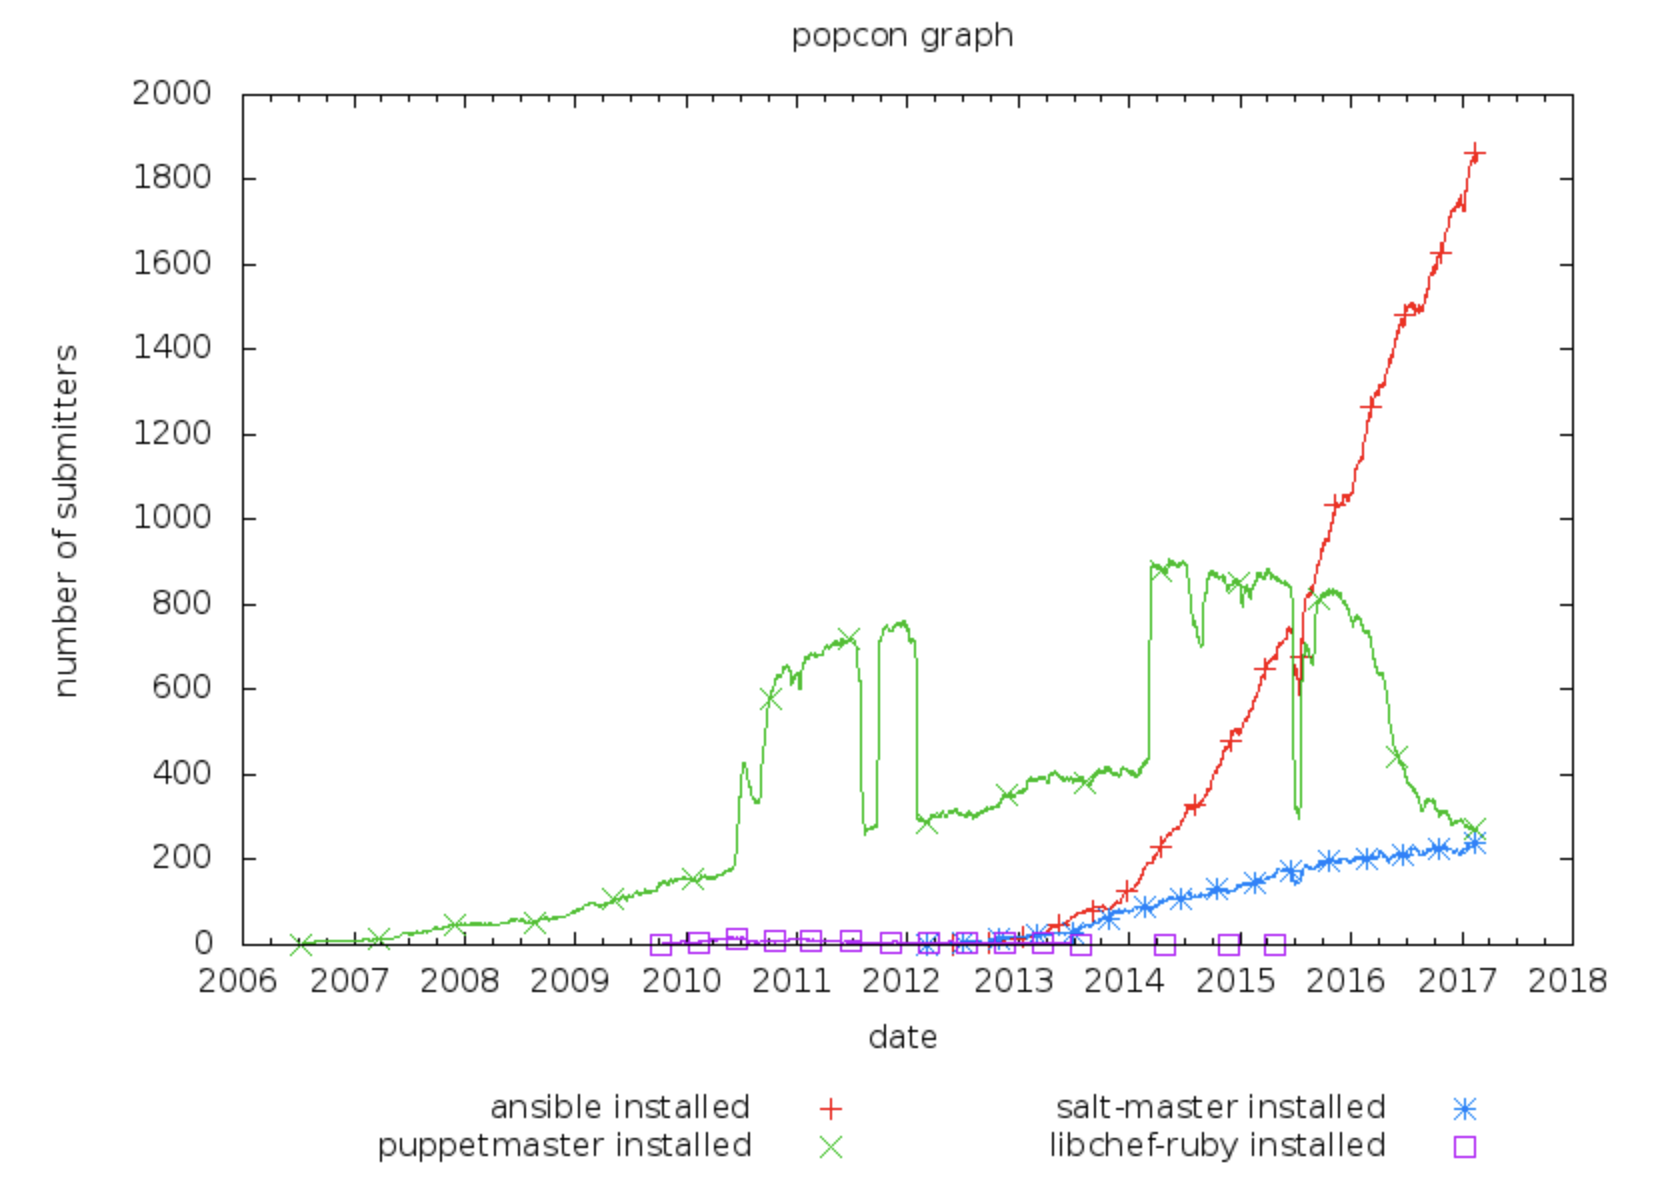
\includegraphics[width=\linewidth]{img/popcon_everybody.png}
  \caption{Deze grafiek toont het aantal keer dat een bepaald softwarepakket ge\"{\i}nstalleerd is op een Debian distributie. \autocite{popcon}}
  \label{fig:popcon_everybody}
\end{figure}

\subsection{Profiel van Puppet}

Puppet werd ontwikkeld in 2005 met als doel het automatiseren van data centers. Om dit te kunnen verwezenlijken maakt Puppet gebruik van  het server/client model. De server wordt in dit model de Puppetmaster genoemd. Dit kunnen er  \'e\'en of meerdere zijn.  De client wordt de Puppetagent genoemd. Zowel op de master als op de agent dient Puppet ge{\"\i}nstalleerd te zijn om te kunnen functioneren. \newline

Wanneer een server zichzelf wenst te configureren dient deze een aanvraag te doen bij de Puppetmaster. De Puppetmaster heeft een manifest die de verschillende soorten configuraties beschrijft. De Puppetmaster gecompileerd vervolgens dit manifest naar een catalogus. Een catalogus is uniek voor elke Puppetagent. Dit komt omdat er bij het compileren van het manifest naar de catalogus rekening gehouden wordt met diverse parameters zoals de functie van de server of de distributie van het besturingssysteem dat op die server draait \autocite{Puppetlanguagecatalog}. Eens de Puppetagent zijn persoonlijke catalogus ontvangen heeft, zal deze voor zichzelf controleren of er verschillen zijn tussen zijn huidige configuratie en de staat die beschreven staat in de catalogus. Indien er afwijkingen zijn, worden deze ook automatisch opgelost. Zie ook \ref{fig:aanvraagCatalogus} \autocite{Puppetdoc} \autocite{puppetfaq}.

\begin{figure}
  \begin{center}
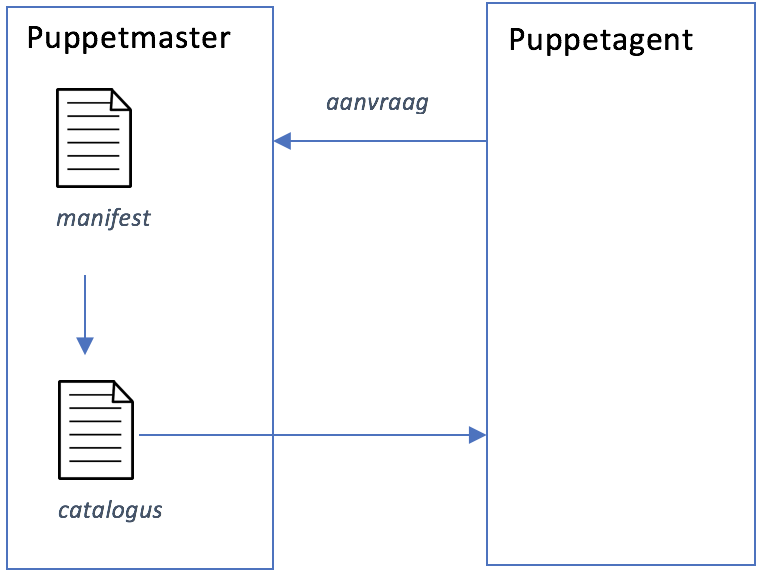
\includegraphics[width=150px]{img/aanvraagCatalogus}
\end{center}  \caption{Aanvraag voor een configuratie}
  \label{fig:aanvraagCatalogus}
\end{figure}


\subsection{Profiel van Ansible}
Ansible is opgericht door Michael DeHaan, iemand die zeer vertrouwd was met Puppet \autocite{ansiblefordevops}. Hij vond dat bedrijven die Puppet gebruikten, moeilijkheden ondervonden op gebied van eenvoud en automatisatie. Daarom is hij samen met Sa{\"\i}d Ziouani Ansible Inc. gestart. \newline

Bij Ansible worden configuraties van een centraal punt genaamd Ansible Tower verstuurd. Ook hier kan voor rendundantie meerdere Ansible Towers aanwezig zijn in de infrastructuur. Het is echter geen verplichting om van een dergelijk centraal punt gebruik te maken. In feite is elke computer waarop Ansible is ge\"installeerd in staat om configuraties uit te voeren. Ansible Tower verstuurd modules naar de te configureren servers, waar ze worden uitgevoerd en vervolgens weer verwijderd. Ook Ansible bezit de functionaliteit om na te gaan of de huidige configuratie in lijn is met de ontvangen modules. \autocite{ansibledoc}.


%% TODO: deze sectie (die je kan opsplitsen in verschillende secties) bevat je
%% literatuurstudie. Vergeet niet telkens je bronnen te vermelden!





\section{Opzet van deze bachelorproef}
\label{sec:opzet-bachelorproef}

In dit onderzoek vallen kleinere CMT's zoals Chef en Salt buiten de scope en zal de focus liggen op Puppet en Ansible. Dit onderzoek vindt plaats op MediaIT, een afdeling binnen VRT zoals weerspiegeld is op het organigram in figuur \ref{fig:organigram} .



Momenteel wordt er gebruik gemaakt van Puppet maar deze voldoet niet aan de verwachtingen van de bussiness en daarom is er dan ook besloten om de huidige Puppet-infrastructuur te vervangen door Ansible.
Deze bachelorproef zal onderzoeken wat er precies misgelopen is en waarom deze problemen zich hebben voorgedaan. Vervolgens zal er gekeken worden of Ansible deze problemen \"uberhaupt kan oplossen. Dit rapport wil een hulp bieden aan bedrijven die dezelfde stappen overwegen zodat het op voorhand duidelijk is wat er verwacht kan worden, wat de mogelijkheden zijn en waar een CMT te kort schiet. Ansible is sinds enige tijd aan een stevige opmars bezig maar er zijn voldoende voorbeelden van opensource (en andere) projecten die na een initi\"ele hype snel in mekaar zakten. Ondertussen heeft Ansible tal van mooie referenties achter zich en heeft het positieve analyses gekregen van belangrijke partijen zoals RedHat en Gartner. Is Ansible echter noemenswaardig beter dan bijvoorbeeld Puppet die reeds een lange bewezen staat van diens heeft (meer dan 12 jaar) en een grote community die het project ondersteunt.


\begin{figure}
  \begin{center}
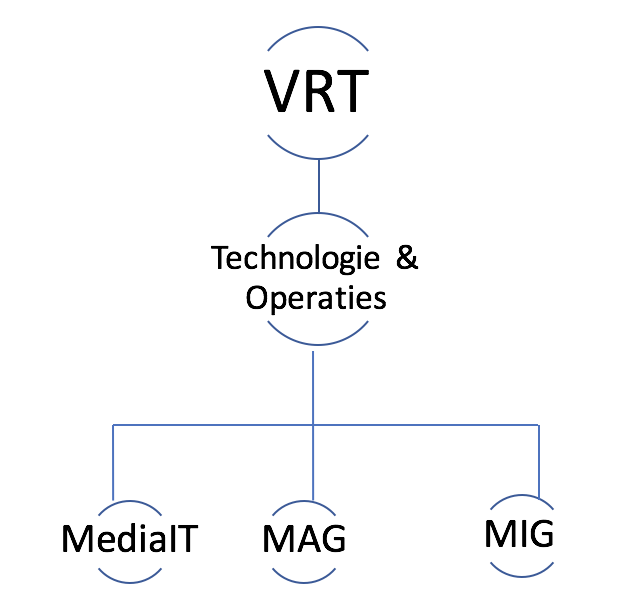
\includegraphics[width=150px]{img/organigram}
\end{center}  \caption{Organigram waarbinnen dit onderzoek zich afspeelt.}
  \label{fig:organigram}
\end{figure}


\section{Probleemstelling en Onderzoeksvragen}
\label{sec:onderzoeksvragen}

%% TODO:
%% Uit je probleemstelling moet duidelijk zijn dat je onderzoek een meerwaarde
%% heeft voor een concrete doelgroep (bv. een bedrijf).
%%
%% Wees zo concreet mogelijk bij het formuleren van je
%% onderzoeksvra(a)g(en). Een onderzoeksvraag is trouwens iets waar nog
%% niemand op dit moment een antwoord heeft (voor zover je kan nagaan).


%% TODO: Het is gebruikelijk aan het einde van de inleiding een overzicht te
%% geven van de opbouw van de rest van de tekst. Deze sectie bevat al een aanzet
%% die je kan aanvullen/aanpassen in functie van je eigen tekst.

De overschakeling van Puppet naar Ansible is geen kleine stap en kan mogelijk voor veel complicaties zorgen. Daarom weet men best op voorhand wat er te wachten staat en zullen er in dit onderzoek verschillende relevante zaken onderzocht worden die kunnen worden opgedeeld in de volgende drie grote categorie\"en. 


\subsection{Wat zijn de redenen van een omschakeling?}

Het is belangrijk te weten wat de drijfveren waren voor de beslissing om Puppet te vervangen door Ansible en dat is precies waar deze eerste categorie toe dient. Om een profiel van de situatie op te kunnen stellen zal een interview plaatsvinden met de verantwoordelijken binnen de VRT om zo te achterhalen waar Puppet te kort schoot en waarom men denkt dat Ansible hier een oplossing biedt. Als bedrijven hun situatie herkennen in dit profiel, is het geadviseerd om te overwegen of een overstap ook voor hen al dan niet aan te raden is.

\subsection{Wat zijn de technische voor-en nadelen van Puppet en Ansible?}

In deze tweede categorie zal er een vergelijkende studie plaatsvinden waarbij technische aspecten zoals performantie, schaalbaarheid en veiligheid vergeleken worden. 
 
 Ten eerste wordt de performantie onderzocht. Hieronder wordt verstaan de tijd die nodig is tot het bekomen van een consistente staat en deze zal onderzocht worden in twee situaties. Bij de eerste is er namelijk nog geen configuratie aanwezig en dient alles nog ge\"installeerd en geconfigureerd te worden. Bij de tweede situatie is er wel al een configuratie aanwezig en is het de bedoeling dat de CMT enkel de nodige aanpassingen doorvoert en niet alles opnieuw configureert. 

Ten tweede is er de schaalbaarheid. Onder schaalbaarheid wordt verstaan: het vermogen om grote vraag te verwerken zonder kwaliteit te verliezen \autocite{informit}. We zullen monitoren hoe Ansible en Puppet hun resources verdelen bij een toenemende drukte, hier onder de vorm van meer servers en uitgebreidere configuraties. 

Er wordt afgesloten met een analyse over de veiligheid. Hierbij zal er een literatuurstudie plaatsvinden met onderzoek naar welke veiligheidsproblemen reeds gekend zijn en wat de impact hiervan is op een bedrijfsnetwerk. CMT's hebben namelijk  administrator rechten tot verschillende servers die ze dienen te configureren. Wanneer de server waarop een CMT draait besmet is, kunnen de gevolgen catastrofaal zijn.

\subsection{Wat is het verloop van een dergelijke transitperiode?}

Problemen die bij de vervanging van Puppet door Ansible optreden, zullen gerapporteerd worden en er zal onderzocht worden waarom deze optraden. Al dan niet gevonden oplossingen zullen beschreven en uitgelegd worden zodat andere bedrijven zich goed bewust zijn van wat er te wachten staat en hoe ze eventueel sommige voorvallen best kunnen oplossen. Welke incidenten zich zullen voordoen, valt uiteraard moeilijk te voorspellen. 

%%In Hoofdstuk~\ref{ch:methodologie} wordt de methodologie toegelicht en worden de gebruikte onderzoekstechnieken besproken om een antwoord te kunnen formuleren op de onderzoeksvragen.

%% TODO: Vul hier aan voor je eigen hoofstukken, één of twee zinnen per hoofdstuk

%%In Hoofdstuk~\ref{ch:conclusie}, tenslotte, wordt de conclusie gegeven en een antwoord geformuleerd op de onderzoeksvragen. Daarbij wordt ook een aanzet gegeven voor toekomstig onderzoek binnen dit domein.

